\subsection{Première partie du transitoire: solidification à l'interface d'un bain oxyde} \label{sect:num1}
Le bain initial correspond à un bain oxyde avec une masse initiale de 10t, une température initiale de 2900 K et une composition en fractions massiques de 0.77 UO$_2$ - 0.12 Zr - 0.11 ZrO$_2$ (ratio molaire $R_{U/Zr}$ = 1.3 et degré  d'oxydation du zirconium $C_{Zr}$ = 30 \%). La puissance résiduelle massique est constante à $200$ W par kg d'uranium. La température de liquidus de l'oxyde est de 3000 K. Les corrélations d'échange de chaleur par les surfaces haute et latérale sont les corrélations Bali (voir~\cite{Bonnet1999} ou~\cite{Tourniaire2009a} pour plus de détails sur les corrélations). Enfin, un profil de flux plat est utilisé pour la distribution latérale de flux de la couche oxyde du bain pour la projection du flux sur les mailles de le croûte (voir section~\ref{sect:couplage}).

La croûte est divisée, tout au long du calcul, en 20 mailles. L'épaisseur de croûte ``résiduelle'' à son apparition est fixée à 5 mm. Une température constante et uniforme de 1600 K est imposée sur les parois extérieures de la croûte (seul le couplage entre le modèle de bain de corium et le modèle de croûte sont testés ici).

Le couplage entre le bain de corium et la croûte est résolu explicitement en temps avec un macro pas de temps de 100 s. Suffisamment de macro pas de temps sont calculés à partir de l'instant initial t = 0 s pour permettre au bain d'atteindre un état thermique quasi-stationnaire.

Durant les différentes étapes du transitoire, de la masse est échangée entre le bain de corium et sa croûte par solidification du bain ou fusion de la croûte. Une attention particulière a été portée pour que le volume de la croûte soit bien pris en compte pour le calcul du volume qu'occupe le bain de corium en fond de cuve de sorte que, le déplacement du niveau haut du bain associé à la solidification/fusion de la croûte (effet de densité) est faible.

La figure~\ref{fig:mass_balance} donne les masses du bain de corium et la masse globale de croûte.
\begin{figure}[H]
\centering
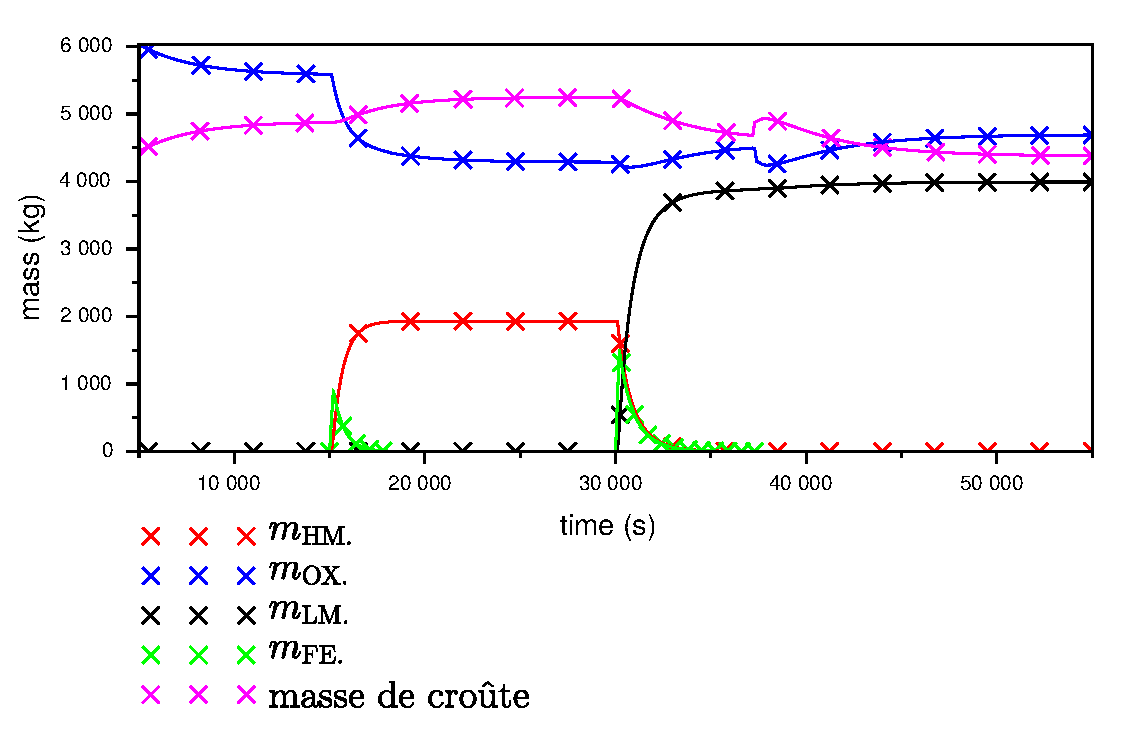
\includegraphics[width=0.85\textwidth, keepaspectratio=true]{Figures/mass_balance.eps}\\
\caption{Masses de la croûte et de la couche oxyde du bain}
\label{fig:mass_balance}
\end{figure}
À chaque macro pas de temps du calcul et en fin de calcul, \emph{on vérifie bien la conservation de la masse globale du système}.

De la même manière, de l'énergie est échangée entre le bain de corium et la croûte et \emph{on vérifie la conservation globale de l'énergie du système}. La figure~\ref{fig:thermal_balance} donne les différentes puissances d'intérêt du bain de corium et de la croûte au cours du transitoire : les puissances évacuées par la surface latérale de la couche oxyde du bain $\bar{\phi}^{lat}_\textrm{OX.}S^{lat}_\textrm{OX.}$ et par sa surface supérieure $\bar{\phi}^{up}_\textrm{OX.}S^{up}_\textrm{OX.}$, la puissance résiduelle de la couche oxyde du bain $Q_\textrm{OX.}$ ainsi que la somme des puissances résiduelles $Q_{C_j}$ des mailles $C_j$ de la croûte, et enfin la somme des puissances $\bar{\phi}_{j,ext}S_{j,ext}$ évacuées par la surface extérieure $\gamma_{ext}$ des mailles $C_j$ de la croûte.
\begin{figure}[H]
\centering
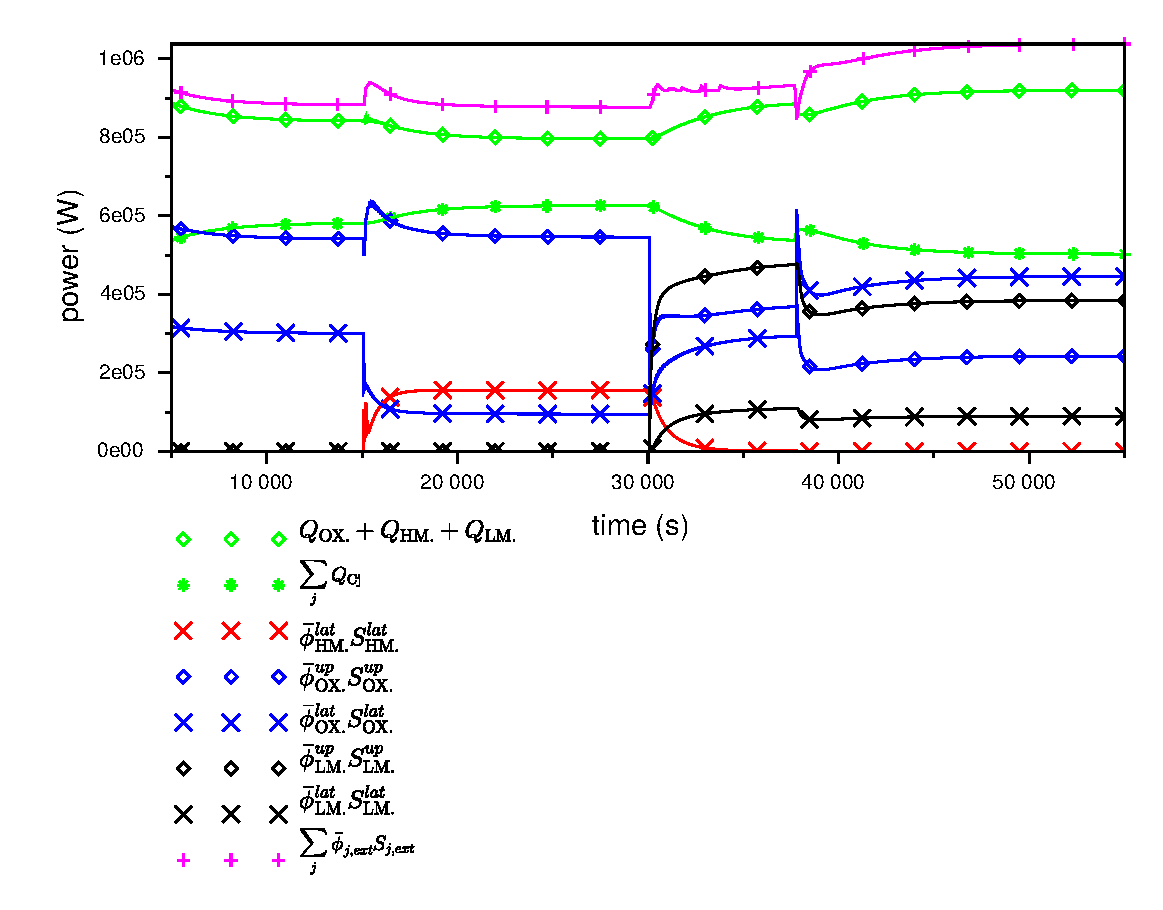
\includegraphics[width=0.85\textwidth, keepaspectratio=true]{Figures/thermal_balance.eps}\\
\caption{Puissances d'intérêt du système bain de corium et croûte}
\label{fig:thermal_balance}
\end{figure}
La conservation de l'énergie peut être vérifiée graphiquement dans la figure~\ref{fig:thermal_balance} à l'état quasi-stationnaire atteint. Pour t=15 000 s, on vérifie bien que
\begin{equation}
\bar{\phi}^{up}_\textrm{OX.}S^{up}_\textrm{OX.} + \bar{\phi}_{j,ext}S_{j,ext} = Q_\textrm{OX.} + \sum_j Q_{C_j}.
\end{equation}

Durant le transitoire du couplage, les mailles de la croûte sont directement en était de solidification (voir la section~\ref{sect:thermique} pour la description des différents états solidification, conduction et fusion). La croûte se solidifie jusqu'à atteindre un état quasi-stationnaire de solidification (voir figure~\ref{fig:croutes_1}) et, conformément au choix d'un profil uniforme de flux, l'épaisseur de la croûte est, elle aussi uniforme.

\begin{figure}[H]
\centering
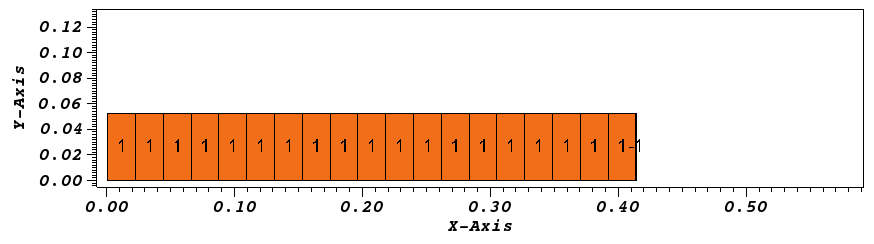
\includegraphics[width=\textwidth, keepaspectratio=true]{Figures/coriumCrust_100.png}\\
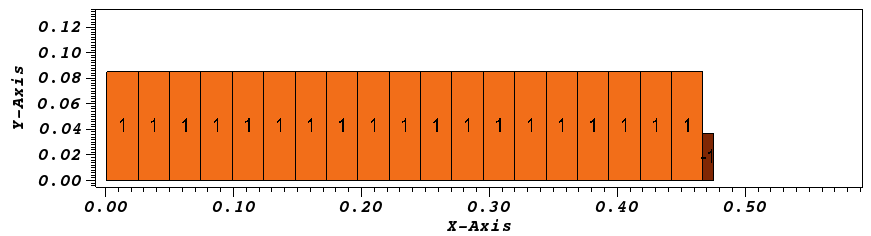
\includegraphics[width=\textwidth, keepaspectratio=true]{Figures/coriumCrust_15000.png}
\caption{Croûte à t = 100 s (en haut) et à t = 15 000 s (en bas). \textit{L'indice dans la maille $C_j$ donne la couche de bain en face de celle-ci : 1 $\Leftrightarrow$ OX., -1 $\Leftrightarrow$ Vide}}
\label{fig:croutes_1}
\end{figure}

\subsection{Seconde partie du transitoire: formation de la couche métallique lourde}

Suite à l'atteinte du régime permanent entre ce bain oxyde et sa croûte, une masse d'acier liquide de 1t est ajoutée au-dessus du bain en continue entre 15000 et 15200 s. La composition associée est, en termes de fractions massiques, 0.687 Fe - 0.208 Cr - 0.106 Ni tandis que la température est de 1605 K. La masse d'acier ajoutée a été selectionnée vis-à-vis du seuil d'inversion de stratification du bain\footnote{correspondant à quantité d'acier dans la bain permettant le passage d'un état d'équilibre thermochimique composé d'une couche métallique lourde en dessous d'une couche oxyde vers un équilibre composé d'une couche oxyde en dessous d'une couche métallique légère} afin d'amener le bain vers un équilibre à deux couches : une couche métallique lourde surmontée d'une couche oxyde.

Dans cette seconde partie du transitoire, les températures de liquidus considérées pour le métal lourd et l'acier sont égales à 1600 K.

Les profils d'épaisseur de la croûte à 15200 s (apparition de la couche métallique lourde) et à 30000 s (état quasi-stationnaire du bain HM./OX.) sont présentés à la figure~\ref{fig:croutes_2}.
A 15200 s, une maille de croûte apparaît en face d'une couche d'acier liquide (à une hauteur h $>$ 0.42 m) provenant de la coulée et le maillage de la croûte oxyde passe de 20 mailles (à t=15 000s) à 19 mailles (à t=15 200s). Cette maille de croûte d'acier apparaît avec une épaisseur initiale de 5 mm mais fond presque instantanément lorsque la couche d'acier s'échauffe. 

A 15200 s, on a aussi apparition de la couche métallique lourde de par le transfert de masse entre couches associé à la cinétique de stratification; par hypothèse de ce modèle, cette couche est formée à la température de la couche oxyde (dans ce cas, 3027 K). Cette couche de bain nouvellement formée est en contact avec la croûte oxyde formée dans la première partie du transitoire. Dans les premiers instants qui suivent, l'épaisseur de ces mailles de croûte reste constante \textit{i.e.} on a un flux transmis par la frontière latérale de cette couche qui est évacué par conduction dans la croûte et la couche métallique se refroidit. Avec un schéma explicite et un pas de temps de 100s., apparaissent alors des oscillations couplées sur la température de la couche HM. d'une part et sur l'état des mailles de la croûte en regard qui passent de ``pure conduction'' (où la température d'interface est calculée par l'égalité des flux de part et d'autre) à ``solidification'' (où la température d'interface est égale à 1600 K, la température de liquidus de HM.) d'autre part. Ces oscillations amènent à une solidification partielle de la couche HM. qui invalide le reste du transitoire. On a, en bas du bain, à 30000 s une croûte d'épaisseur stabilisée à 10.5cm, soit environ 2cm de plus que son épaisseur à 15 000 s alors que l'on s'attendait ce que les mailles de croûte restent stables en masse. On peut noter que, cette solidification ``parasite'' et les effets de niveau des couches du bain conduisent à des mailles de croûtes avec une composition moyenne variable axialement de telle sorte que, à 30000 s., en face de la couche oxyde, l'épaisseur de croûte n'est pas constante en partie basse de la couche (la croûte plus ``métallique'' en bas a une conductivité plus grande et amène, à flux donné, en régime permanent, à une épaisseur plus importante). Par ailleurs, les oscillations en températures de la couche HM. ont une amplitude de l'ordre de 600K qui ne décroit pas dans le temps.

En bref, le schéma de couplage entre bain et croûte pose problème à l'apparition d'une phase métallique liquide à l'interface d'une croûte oxyde.

\begin{figure}[H]
\centering
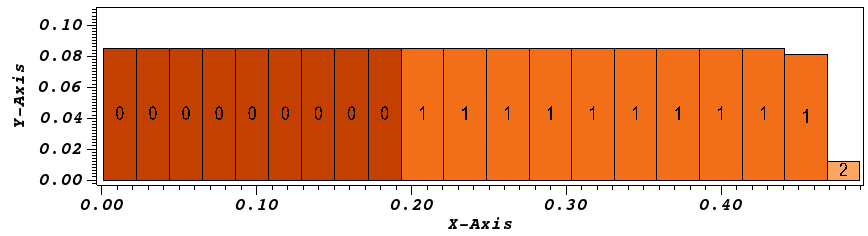
\includegraphics[width=\textwidth, keepaspectratio=true]{Figures/coriumCrust_15200.png} \\
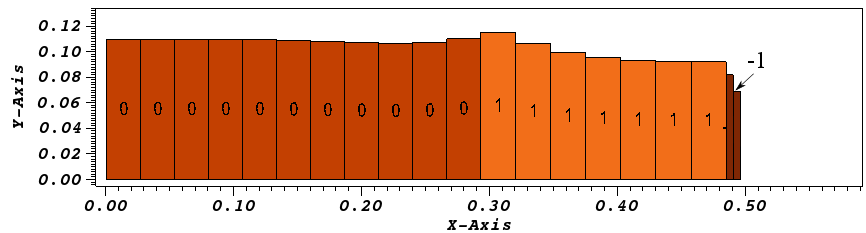
\includegraphics[width=\textwidth, keepaspectratio=true]{Figures/coriumCrust_30000.png}
\caption{De haut en bas, croûte à t=15 200 s (apparition de la couche métallique lourde), t=30 000 s (état quasi-stationnaire du bain HM./OX.). \textit{L'indice dans la maille $C_j$ donne la couche de bain en face de celle-ci : 0 $\Leftrightarrow$ HM., 1 $\Leftrightarrow$ OX.}, 2  $\Leftrightarrow$ FE., -1 $\Leftrightarrow$ aucune couche de bain}
\label{fig:croutes_2}
\end{figure}

\subsection{Tests de vérification à venir}

Le problème d'oscillations rencontré va bien sûr être analysé dans l'objectif de le corriger pour fournir une première version satisfaisante du modèle dans la prochaine livraison de PROCOR.

Tout d'abord, notons que les oscillations rencontrées de l'état des mailles de la croûte (entre ``pure conduction'' et ``solidification'') sont liées au choix de modélisation de distinguer \textit{a priori} des températures de solidification $\temperature[sol]{l(j)}$ et de fusion $\temperature[fus]{j}$ (dans le transitoire précédent, la croûte oxyde refond à 3000 K tandis que la couche HM. se solidifie à 1600 K). Si, comme dans les hypothèses de macroségrégation initiales du modèle de bain de PROCOR, on considère une unique température d'interface associée à la température de liquidus globale, ces oscillations sont supprimées et le modèle est fonctionnel.

Bien sûr, ce problème est lié au schéma en temps de couplage (en l'occurence explicite avec un macro pas de temps assez grand) mais il est compliqué par l'utilisation de fermetures (en l'occurence, pour traiter la conduction radiale dans la croûte) qui propagent l'information instantanément par suppression de la composante spatiale dans les équations de ce type de modèle intégral \cite{Viot2018}. Ainsi, l'hypothèse d'un profil quadratique à tout instant dans l'épaisseur de chaque maille de croûte peut amener à des changements de convexité non-physiques du profil de température pour certaines discontinuités des conditions aux limites (voir \cite{Peybernes2018}).

Ainsi, pour avancer, l'utilisation d'un schéma implicite, tel qu'offert par les fonctionnalités de l'architecture développée dans le cadre de la thèse de Louis Viot \cite{Viot2018}, va être testée. Par ailleurs, pour bien cartographier les problèmes éventuels relatifs au traitement de la conduction, un cas test plus unitaire va être mis en place. Il consiste à simplifier le transitoire précédent.
Partant d'une configuration stationnaire entre un bain oxyde et sa croûte (réduite à une seul maille)\footnote{Le transitoire relatif à la solidification à l'interface un bain oxyde a, lui, bien été validé (\textit{cf.} \Sect{num1}).}, la phase oxyde liquide est instantanément ``remplacée'' par une phase métallique de température de liquidus bien inférieure. Ce test sera paramétrique vis-à-vis de la masse initiale de la phase métallique et permettra de faire la part des choses entre artefact numérique dû au schéma de couplage et problème de modélisation. Pour ce dernier point, on peut d'ores et déjà anticiper un problème pour une masse trop faible de métal qui conduirait à une inversion du flux de chaleur à l'interface (\textit{i.e.} c'est la croûte qui chauffe le liquide) qui n'est pas compatible avec les fermetures du bilan thermique de cette couche.
